\subsection{Transfer matrix model}
The transfer matrix model is used for simulating external light incident on the device. It assumes light hits the device normal to the surface.  The model can can calculate 

\begin{figure}[H]
\centering
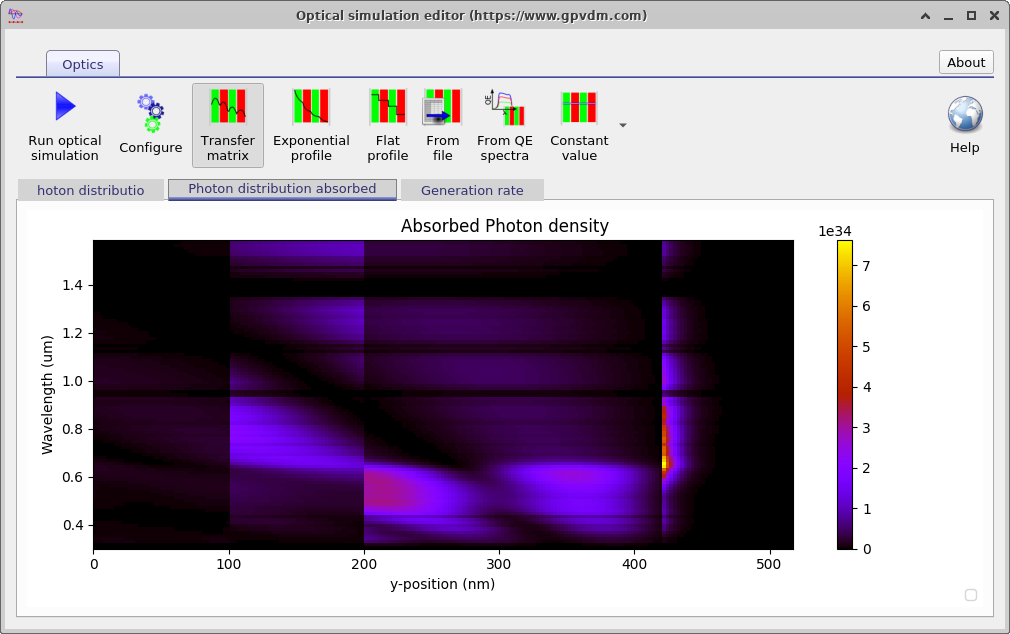
\includegraphics[width=1.0\textwidth,height=0.6\textwidth]{./images/opticalsimulation4.png}
\caption{The output tab this is just like windows file explorer, you can explore the simulation directory tree.}
\label{fig:transfermatrix0}
\end{figure}

\begin{figure}[H]
\centering
\begin{tabular}{ c c }

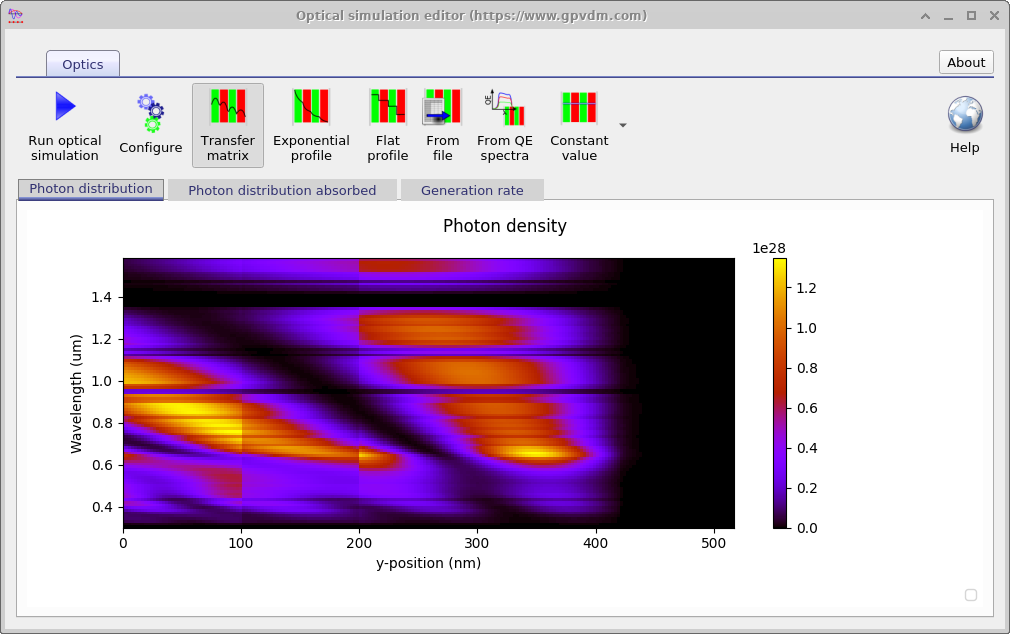
\includegraphics[width=0.5\textwidth,height=0.4\textwidth]{./images/opticalsimulation.png}

&
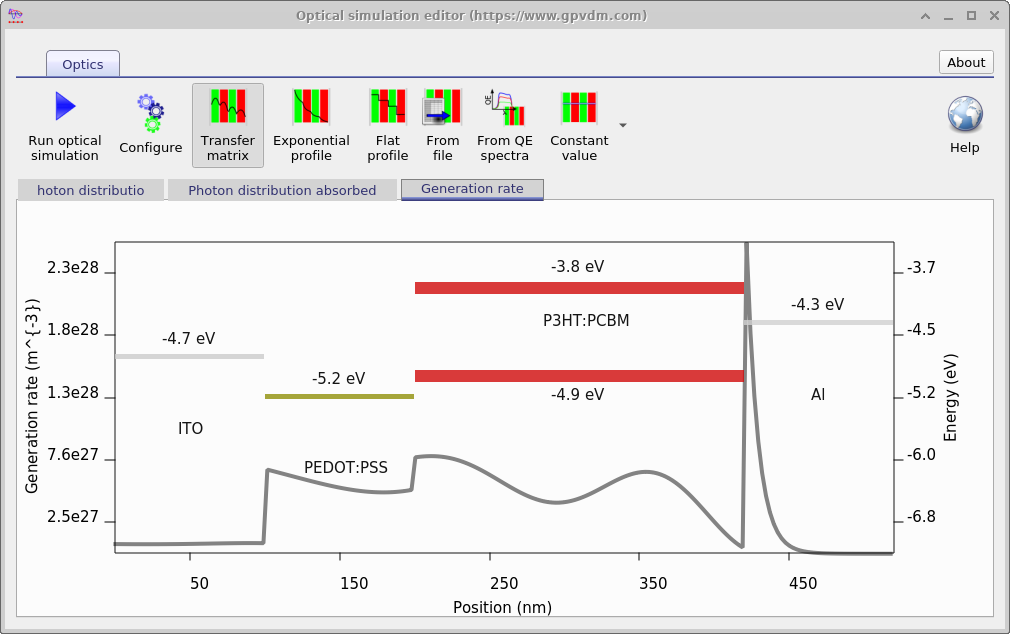
\includegraphics[width=0.5\textwidth,height=0.4\textwidth]{./images/opticalsimulation1.png}

\\
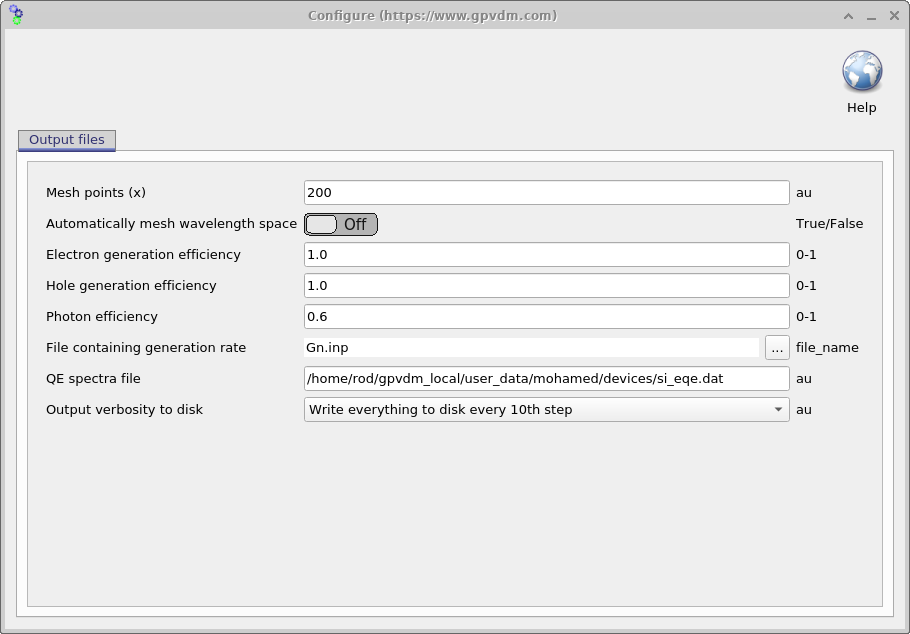
\includegraphics[width=0.5\textwidth,height=0.4\textwidth]{./images/opticalsimulation2.png}

&
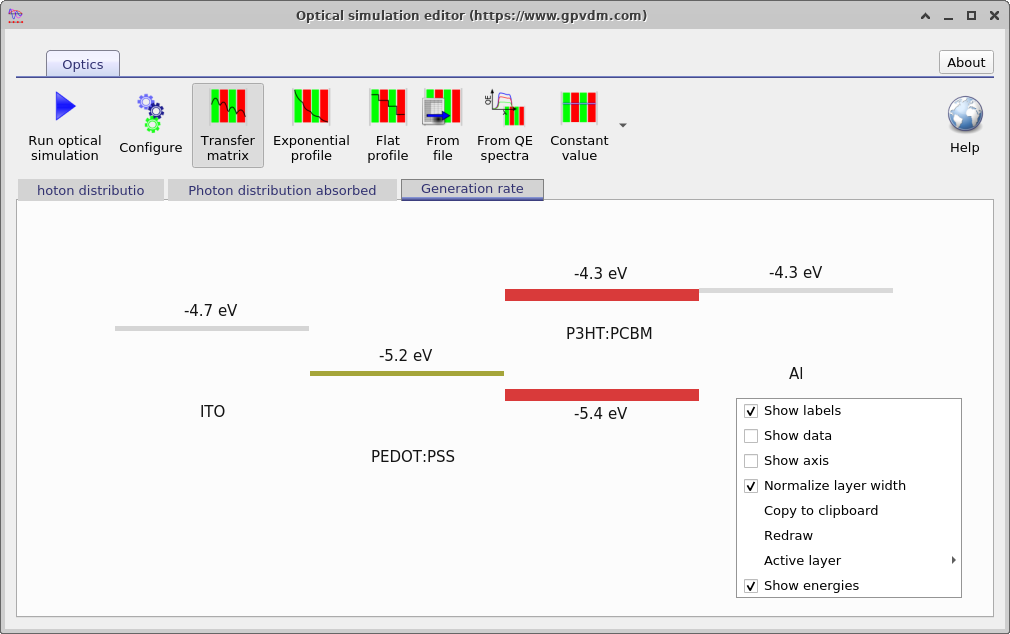
\includegraphics[width=0.5\textwidth,height=0.4\textwidth]{./images/opticalsimulation3.png}

\\
\end{tabular}
\caption{The optical simulation window}
\label{fig:transfermatrix1}
\end{figure}



\subsubsection{Theory}
On the left of the interface the electric field is given by

\begin{equation}
E_{1}=E^{+}_{1} e^{-j k_1 z}+E^{-}_{1} e^{j k_1 z}
\label{efield1}
\end{equation}
and on the right hand side of the interface the electric field is given by
\begin{equation}
E_{2}=E^{+}_{2} e^{-j k_2 z}+E^{-}_{2} e^{j k_2 z}
\label{efield2}
\end{equation}

Maxwel's equations give us the relationship between the electric and magnetic fields for a plane wave.

\begin{equation}
\nabla \times E=-j\omega \mu H 
\end{equation}
which simplifies to:
\begin{equation}
\frac{\partial E} {\partial z}=-j\omega \mu H 
\label{maxwel}
\end{equation}

Applying equation \ref{maxwel} to equations \ref{efield1}-\ref{efield2}, we can get the magnetic field on the left of the interface
\begin{equation}
-j \mu \omega H^{y}_{1}=-j k_1 E^{+}_{1} e^{-j k_1 z}+j k_1 E^{-}_{1} e^{j k_1 z}
\end{equation}
and on the right of the interface
\begin{equation}
-j \mu \omega H^{y}_{2}=-j k_2 E^{+}_{2} e^{-j k_2 z}+j k_2 E^{-}_{2} e^{j k_2 z}.
\end{equation}

Tidying up gives,
\begin{equation}
H^{y}_{1}=\frac{k}{\omega \mu}E^{+}_{1} e^{-j k_1 z}-\frac{k}{\omega \mu} E^{-}_{1} e^{j k_1 z}
\end{equation}

\begin{equation}
H^{y}_{2}=\frac{k}{\omega \mu}E^{+}_{2} e^{-j k_2 z}-\frac{k}{\omega \mu} E^{-}_{2} e^{j k_2 z}
\end{equation}


\subsubsection{Refractive index and absorption}
\begin{equation}
E(z,t)=Re(E_0 e^{j(-kz+\omega t)})= Re(E_0 e^{j(\frac{-2 \pi (n+j\kappa)}{\lambda}z + \omega t)})=e^{\frac{2\pi\kappa z}{\lambda}}Re(E_0 e^{\frac{j(-2 \pi (n+j\kappa)}{\lambda}z +\omega t})
\end{equation}
And because the intensity is proportional to the square of the electric field the absorption coefficient becomes

\begin{equation}
e^{-\alpha x}=e^{\frac{2\pi\kappa z}{\lambda}}
\end{equation}

\begin{equation}
\alpha=-\frac{4\pi\kappa}{\lambda_0}
\end{equation}

\subsubsection{Local ground view factor}
The local ground view factor is given as \cite{neryterrain}

\begin{equation}
F_{ground}=sin^2 \left ( \frac{\theta_t}{2}\right )=\frac{1-cos(\theta_t)}{2}
\end{equation}


\subsubsection{Meshing}
The optical mesh automatically extends to cover the optical simulation window, so one does not usually need to worry about configuring it.  The optical material layers are defined in the list at the bottom of figure \ref{fig:emesh}.  The first column is a unique identifier, it must start with a hash symbol, but apart from that you can call it what you want.  The second column is the thickness of the layer.  The forth column is the material system, data files describing the material system are stored in the 'phys' directory.  Finally, the forth column tells the model if the layer is part of the active layer or not (more about that in the next section.)



\subsubsection{Interfacing the electrical and optical models}
In gpvdm there is both an electrical model and an optical model.  The optical simulation usually includes the glass substrate, the contacts and layers such as PEDOT:PSS.  The electrical simulation usually only covers the active layer of the device, thus a typically optical simulation is much bigger than the electrical simulation window.  The optical model feeds the calculated optical profile of the light into the electrical simulation.  You must therefore tell the optical model which layer in the optical simulation represents the active layer.  This is done by placing a 'yes' in the column 'Active layer' in figure \ref{fig:opticalsimulation}.
\newpage
\vfill

